\subsection{UC1 - Inserimento dei dati }
\label{uc1}

    \begin{figure}[htbp]
        \centering
        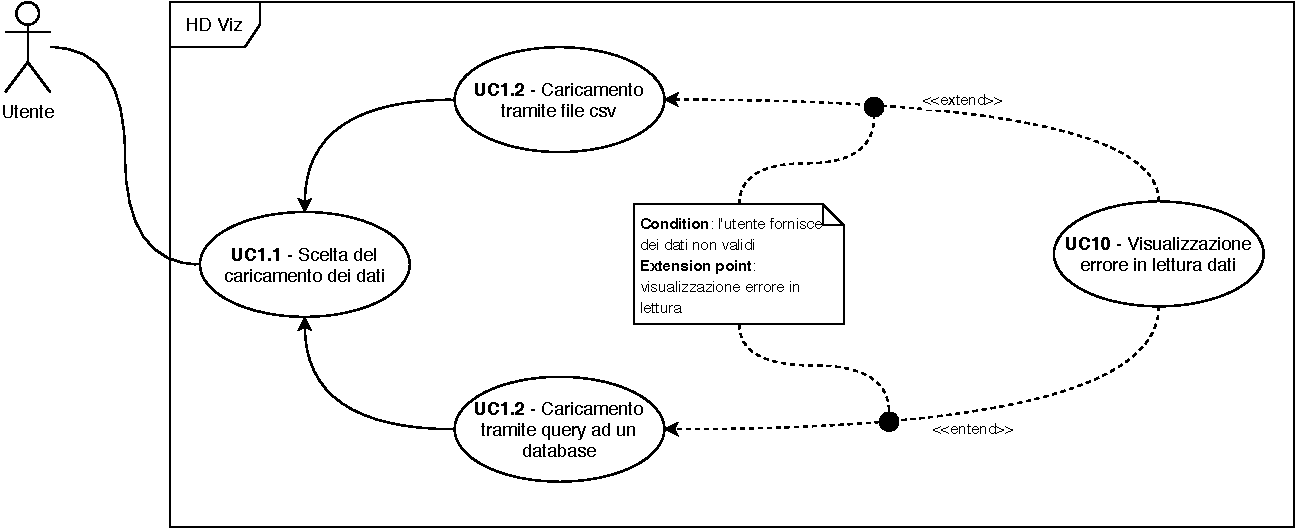
\includegraphics[width=1.0\textwidth]{source/sections/casi-uso/diagrams/uc1.pdf}
        \caption{UC1 - Inserimento dei dati}
        % \label{fig:uc1}
    \end{figure}
    
    \begin{itemize}
    \item \textbf{Attore}: utente;
    \item \textbf{Descrizione}: l'utente carica i dati per ottenere una visualizzazione;
    \item \textbf{Precondizione}:
    \begin{itemize}
        \item il sistema è funzionante e raggiungibile;
        \item l'utente accede alla pagina dell'applicazione.
    \end{itemize}
    \item \textbf{Postcondizione}: i dati sono stati caricati correttamente come matrice $N\times M$;
    \item \textbf{Scenario Principale}: 
        \begin{enumerate}
            \item l'utente accede alla pagina dell'applicazione;
            \item l'utente sceglie come caricare i dati:
                \begin{enumerate}
                    \item l'utente ha scelto di ricavare i dati caricando un file csv;
                    \item l'utente ha scelto di ricavare i dati tramite una query a un database.
                \end{enumerate}
        \end{enumerate}  
    \item \textbf{Estensioni}:
        \begin{enumerate}
            \item l'utente inserisce dei dati non validi o non nel formato corretto:
                \begin{enumerate}
                    \item fallisce l'inserimento dei dati;
                    \item viene visualizzato un messaggio di errore in lettura dei dati (\hyperref[uc10]{UC10}).
                \end{enumerate}
        \end{enumerate}  
    \item \textbf{Generalizzazioni}:
        \begin{enumerate}
            \item l'utente sceglie come caricare i dati:
                \begin{enumerate}
                    \item caricando un file csv (\hyperref[uc1.1]{UC1.1});
                    \item caricamento di una tabella di un database (\hyperref[uc1.2]{UC1.2}).
                \end{enumerate}
        \end{enumerate}  
    \end{itemize}
    
    %%%
    \subsubsection{UC1.1 - Caricamento tramite file csv}
    \label{uc1.1}
    
    \begin{itemize}
    \item \textbf{Attore}: utente;
    \item \textbf{Descrizione}: l'utente sceglie di caricare i dati tramite un file csv;
    \item \textbf{Precondizione}:
    \begin{itemize}
        \item il sistema è funzionante e raggiungibile;
        \item l'utente accede alla pagina dell'applicazione;
        \item l'utente è in possesso di un file csv contenete i dati.
    \end{itemize}
    \item \textbf{Input}: file csv contenente i dati da visualizzare;
    \item \textbf{Postcondizione}: l'utente ha caricato il suo file csv come matrice $N\times M$;
    \item \textbf{Scenario Principale}: 
        \begin{enumerate}
            \item l'utente ha scelto di inserire i file tramite un file csv;
            \item tramite l'apposito bottone sceglie il file.
        \end{enumerate}
        \item \textbf{Estensioni}:
        \begin{enumerate}
            \item l'utente inserisce dei dati non validi o non nel formato corretto:
                \begin{enumerate}
                    \item fallisce l'inserimento dei dati;
                    \item viene visualizzato un messaggio di errore in lettura dei dati. (\hyperref[uc10]{UC10}):
                \end{enumerate}
        \end{enumerate}  
    \end{itemize}

    
    %%%
    \subsubsection{UC1.2 - Caricamento di una tabella di un database}
    \label{uc1.2}
    
    \begin{itemize}
    \item \textbf{Attore}: utente;
    \item \textbf{Descrizione}: l'utente sceglie di caricare i dati tramite una tabella di un database;
    \item \textbf{Precondizione}:
    \begin{itemize}
        \item il sistema è funzionante e raggiungibile;
        \item l'utente accede alla pagina dell'applicazione;
        \item l'utente ha correttamente creato un file di configurazione dei database all'interno del server
    \end{itemize}
    \item \textbf{Postcondizione}: l'utente si è collegato al database e ha recuperato i dati dalla tabella del database come matrice $N\times M$;
    \item \textbf{Scenario Principale}: 
        \begin{enumerate}
            \item l'utente sceglie di caricare i dati tramite una tabella di un database;
            \item l'utente seleziona la tabella di uno dei database correttamente configurati.
        \end{enumerate}
        \item \textbf{Estensioni}:
        \begin{enumerate}
            \item l'utente inserisce dei dati non validi o non nel formato corretto:
                \begin{enumerate}
                    \item fallisce l'inserimento dei dati;
                    \item viene visualizzato un messaggio di errore in lettura dei dati (\hyperref[uc10]{UC10}).
                \end{enumerate}
        \end{enumerate}  
    \end{itemize}

    